\documentclass[journal]{IEEEtran}
\usepackage[spanish]{babel}
\usepackage[utf8]{inputenc}
\usepackage{enumerate}
\usepackage{graphicx}
\usepackage{booktabs}
\usepackage{physics}

\hyphenation{op-tical net-works semi-conduc-tor}


\begin{document}
\title{Reporte de Práctica: Movimiento Rectilíneo Uniformemente Acelerado}

\author{Licenciatura en Física	\\
Universidad Nacional Autónoma de México - Facultad de Ciencias\\
Profesor: José Alfredo Morales Pérez\\
Ayud. Lab.	Miranda García Ávila\\
Integrantes: Jeshua Roberto Estrada Ocampo,~\IEEEmembership{424003085}\\

            
\thanks{}% <-this % stops a space
\thanks{}% <-this % stops a space
\thanks{}}

\markboth{Laboratorio de Mecánica}%
{Shell \MakeLowercase{\textit{et al.}}: Bare Demo of IEEEtran.cls for Journals}

\maketitle

\begin{abstract}
En esta práctica de laboratorio, se investigó el movimiento rectilíneo uniformemente acelerado (MRUA). Se llevaron a cabo experimentos utilizando una riel de aire inclinado y un deslizador, midiendo el tiempo que tardaba este en recorrer diferentes distancias. Los datos obtenidos se analizaron para determinar la aceleración constante del carro. Los resultados confirmaron la relación teórica entre la distancia recorrida, el tiempo y la aceleración, validando las ecuaciones del MRUA. Este experimento permitió comprender mejor los conceptos de aceleración.
\end{abstract}

\begin{IEEEkeywords}
Movimiento rectilíneo uniformemente acelerado (MRUA), Aceleración, Tiempo, Distancia, 
\end{IEEEkeywords}

\IEEEpeerreviewmaketitle

\section{INTRODUCCIÓN}
\subsection{Planteamiento}

\IEEEPARstart  {E}l estudio del movimiento rectilíneo uniformemente acelerado (MRUA) es fundamental en la física clásica, ya que describe cómo se comportan los objetos en movimiento bajo una aceleración constante. Este tipo de movimiento es común en diversas situaciones cotidianas y tecnológicas, desde la caída de objetos bajo la influencia de la gravedad hasta el comportamiento de vehículos en una pista. Comprender el MRUA permite a los estudiantes y profesionales de la física e ingeniería analizar y predecir el comportamiento de sistemas físicos con precisión. La práctica de laboratorio sobre MRUA no solo refuerza los conceptos teóricos aprendidos en clase, sino que también proporciona habilidades prácticas en la medición y análisis de datos experimentales. Esta práctica es crucial para desarrollar una comprensión profunda y aplicada de los principios de la cinemática y la dinámica.\\

\subsubsection{Objetivos Generales}

 -Comprobar experimentalmente las características del movimiento rectilíneo uniformemente acelerado y validar las ecuaciones que lo describen.\\

\subsubsection{Objetivos particulares}
- Medir el tiempo que tarda un carro en recorrer diferentes distancias en una rampa inclinada.\\
- Calcular la aceleración del carro utilizando los datos obtenidos.\\
- Comparar los resultados experimentales con los valores teóricos esperados.\\
- Analizar posibles fuentes de error en el experimento y evaluar su impacto en los resultados.\\

\subsubsection{Hipótesis}
El movimiento de un carro en una rampa inclinada, bajo condiciones controladas, sigue las leyes del movimiento rectilíneo uniformemente acelerado, y la aceleración del carro será constante e igual a la aceleración teórica calculada.\\

\section{MARCO TEÓRICO}
El estudio del movimiento rectilíneo uniformemente acelerado (MRUA) es una parte integral de la cinemática, que es la rama de la física que describe el movimiento de los cuerpos sin considerar las fuerzas que lo causan. 
El MRUA es un tipo de movimiento en el cual un objeto se desplaza en línea recta con una aceleración constante. Esto significa que la velocidad del objeto cambia uniformemente con el tiempo.
La aceleración (a) se define como el cambio de velocidad (\(\Delta V\)) por unidad de tiempo (\(\Delta t\))

\begin{equation}\label{eq:1}
 a = \frac{v-v_0}{t}
\end{equation}
Despejando la velocidad final (v):
\begin{equation}\label{eq:2}
 v=v_o + ta
\end{equation}

donde v y \(v_o\) son la velocidad final e inicial respectivamente, a es la aceleración, t es el tiempo transcurrido durante el movimiento.

La posición (x) de un objeto en movimiento puede expresarse integrando la ecuación de la velocidad. Partiendo de que la velocidad es la derivada de la posición respecto al tiempo:

\begin{equation}\label{eq:2}
 v = \frac{dx}{dt}
\end{equation}
sustuyendo en la ecuación anterio:

\begin{equation}\label{eq:2}
\frac{dx}{dt} = v_o + ta
\end{equation}

integrando respecto al tiempo: 

\begin{equation}\label{eq:2}
x = x_0 + v_0t + \frac{1}{2}at^2
\end{equation}

donde x y \(x_0\) es la posición final e inicial respectivamente.\\

Tambien está la ecuación de la velocidad en función de la posición, esta ecuación se obtiene combinando las dos anteriores y es útil cuando no se dispone del tiempo:

\begin{equation}\label{eq:2}
v^2 = v_0^2 + 2a(x-x_0)
\end{equation}

En el experimento, un deslizador se desplaza por un riel inclinado. La aceleración del carro en la rampa se debe a la componente de la gravedad en la dirección de la rampa. La aceleración teórica puede calcularse utilizando la inclinación de la rampa y la aceleración debida a la gravedad (g):

\begin{equation}\label{eq:2}
a = g\sin\vartheta
\end{equation}

donde g es la aceleración de la gravedad cuyo valor para este reporte será de  \(9.8 \frac{m}{s^{2}}\).y donde \(\vartheta\) es el ángulo de inclinacion del riel.

\section{ MATERIALES}
\begin{itemize}
\item Riel de baja fricción \item deslizador \item Flexómetro \item Tripie \item Camara de celular \item Software de análisis de video Tracker

\end{itemize}

\section{DESARROLLO EXPERIMENTAL}
\begin{figure}[h]
    \centering
    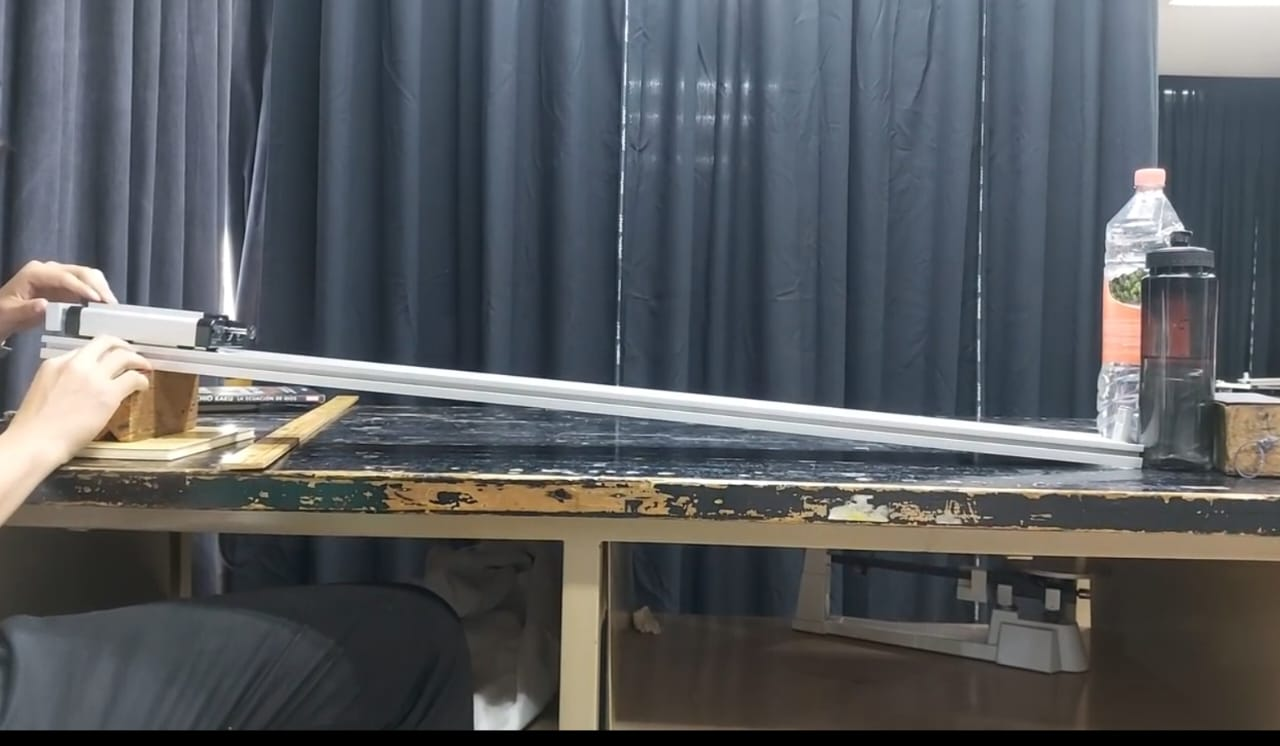
\includegraphics[width=1\linewidth]{inclined.png}
    \caption{Riel de aire inclinado $\vartheta$ grados}
    \label{fig:enter-label}
\end{figure}\\
Para asegurar la validez de los resultados obtenidos en el experimento de movimiento rectilíneo uniformemente acelerado (MRUA), es fundamental establecer condiciones ideales. Estas condiciones incluyen la minimización de la fricción y la reducción de otras fuerzas no deseadas que puedan afectar el movimiento del objeto. Además, es crucial utilizar instrumentos de medición precisos y calibrados.Las condiciones ideales para realizar este experimento son las siguientes:

- Superficie Lisa y Plana: Utilizar un riel de baja fricción sobre una superficie plana para minimizar las fuerzas de fricción que puedan alterar el movimiento del deslizador.\\
- Inclinación Controlada: Añadir una pendiente al riel de manera uniforme utilizando soportes ajustables para mantener un ángulo de - inclinación constante y bien definido.\\
- Manejo de la Iniciación del Movimiento: Asegurarse de que el deslizador se inicie desde el reposo y en el mismo punto de referencia en cada repetición del experimento.\\
Medición Precisa del Tiempo: Utilizar dispositivos de cronometraje con alta precisión, como cronómetros digitales o grabaciones de video que permitan un análisis cuadro por cuadro.\\

Preparación del Equipo:

Colocar un riel de baja fricción sobre una superficie plana y asegurarse de que esté nivelado.
Utilizar soportes ajustables para inclinar el riel a diferentes ángulos. Asegurarse de medir y ajustar el ángulo de inclinación con precisión utilizando un transportador o un inclinómetro.\\

Configuración del Punto de Referencia:

Definir el origen del sistema de referencia \(x_0\) en la parte superior del riel, donde el deslizador comenzará su movimiento.\\

Ejecución del Experimento:

Situar el deslizador en el punto de referencia y soltarlo desde el reposo, permitiendo que se desplace a lo largo del riel inclinado hasta el extremo opuesto.
Grabar el movimiento del deslizador utilizando una cámara de alta velocidad para capturar los tiempos y las distancias recorridas con precisión.
Repetir el procedimiento para diferentes ángulos de inclinación del riel, asegurándose de realizar múltiples pruebas para cada ángulo para obtener datos consistentes y reproducibles.\\
\hfill 

\section{RESULTADOS Y DISCUSIÓN}

\begin{figure}[h]
    \centering
    
\includegraphics[width=1\linewidth]{graph1.png}
    \caption{Diagrama del riel}
    \label{fig:enter-label}
\end{figure}\\\\

Utilizando el coeficiente de correlación lineal de Pearson cada ángulo de inclinación presenta un índice de 99\%, además al graficar distancia contra tiempo cuadrado la gráfica presenta un comportamiento altamente lineal nótese en las siguientes gráficas.\\

\newpage
\begin{figure}[h]
    \centering
    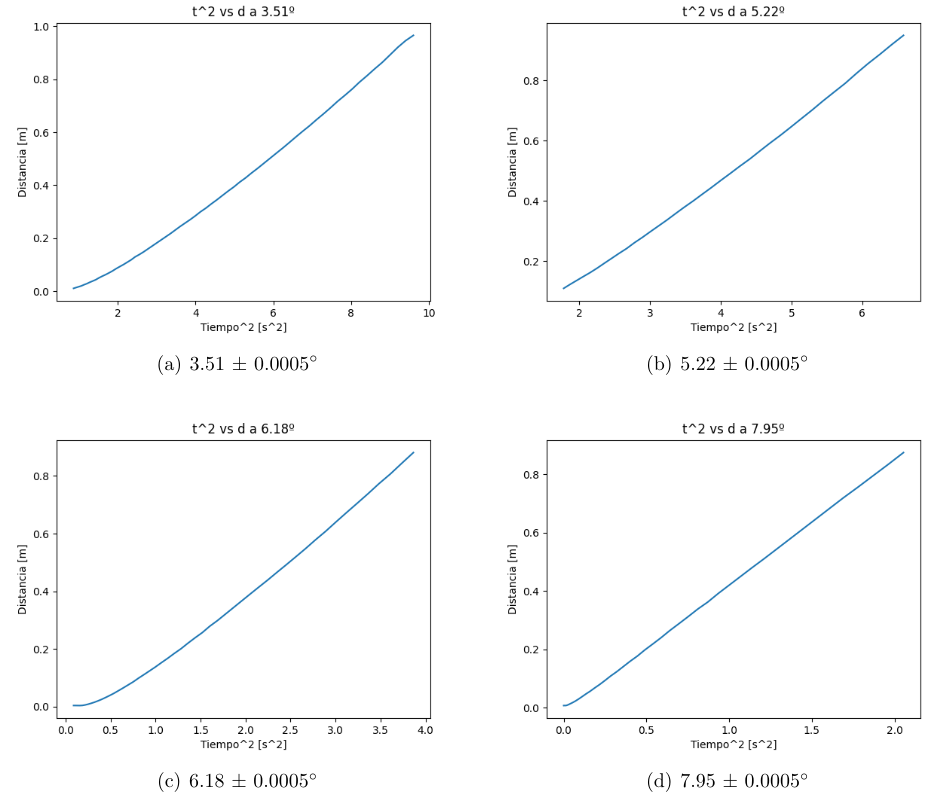
\includegraphics[width=1\linewidth]{graphst^2.png}
    \caption{Distancia vs tiempo cuadrado}
    \label{fig:enter-label}
\end{figure}\\\\



Al graficar distancia contra tiempo obtenemos una función cuadrática, esto es evidente pues es un movimiento uniformemente acelerado por lo que existe una función cuadrática del tiempo que es influenciada por la aceleración gravitacional parcial. \\\\

\begin{figure}[h]
    \centering
    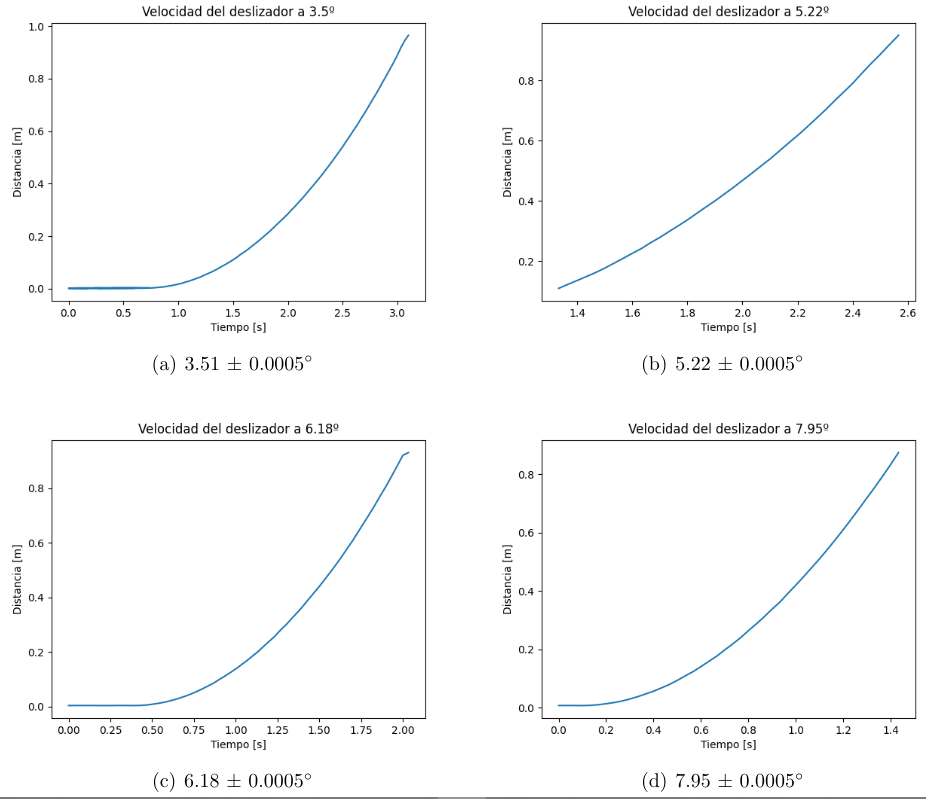
\includegraphics[width=1\linewidth]{d vs t.png}
    \caption{Distancia vs tiempo con incertidumbres de ángulos}
    \label{fig:enter-label}
\end{figure}\\

A continuación se adjuntan las mejores gráficas lineales que se adecuan con el menor grado de incertidumbre a cada una de las gráficas distancias vs tiempo cuadrado:
\newpage

\begin{figure}[h]
    \centering
    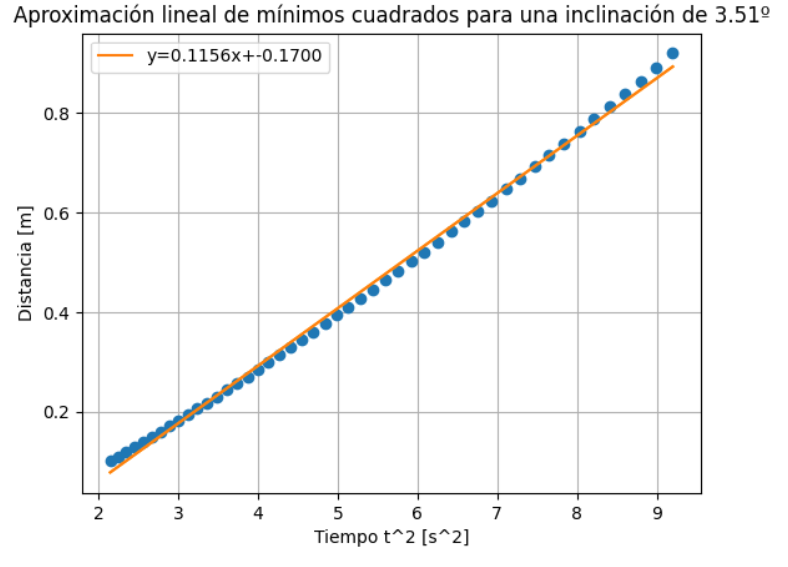
\includegraphics[width=0.9\linewidth]{1er g.png}
    \caption{Mejor gráfica ángulo 1}
    \label{fig:enter-label}
\end{figure}\\

\begin{figure}[h]
    \centering
    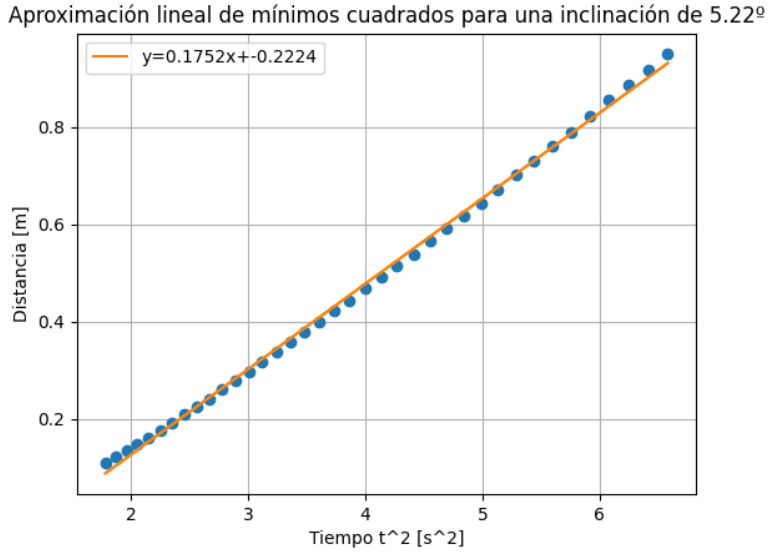
\includegraphics[width=0.9\linewidth]{2do g.png}
    \caption{Mejor gráfica ángulo 2}
    \label{fig:enter-label}
\end{figure}\\

\begin{figure}[h]
    \centering
    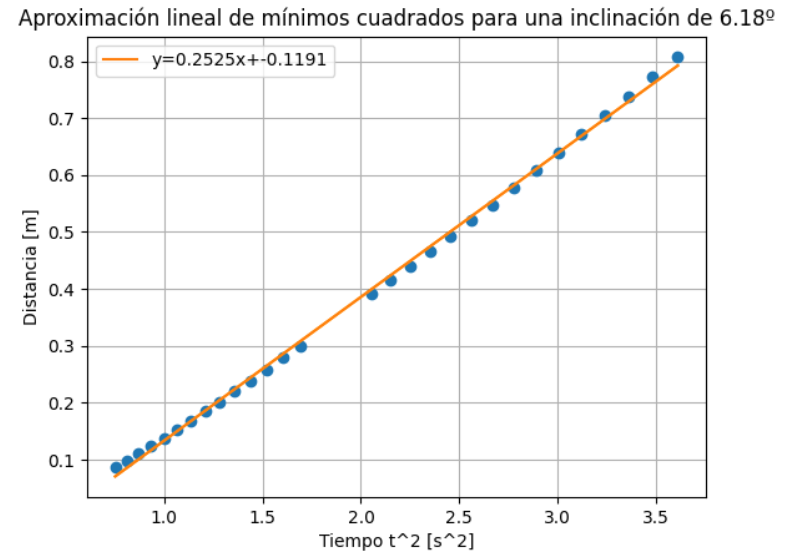
\includegraphics[width=0.9\linewidth]{3er g.png}
    \caption{Mejor gráfica ángulo 3}
    \label{fig:enter-label}
\end{figure}

\section{ CONCLUSIONES} 
Se logró establecer una relación lineal entre el desplazamiento y el cuadrado del tiempo. No obstante, los resultados obtenidos no se aproximaron totalmente al dato teórico, ya que en los cuatro casos con distintos ángulos, la discrepancia con respecto al dato teórico superó el 27\%. Esto podría atribuirse a varios factores: el riel utilizado no era uno de aire, lo cual podría haber introducido fricción, y también a la forma en que se midieron los datos en el software Tracker. En algunos casos, el programa no logró obtener ciertos datos automáticamente, por lo que se tuvo que utilizar otra masa puntual como referencia. Además, la metodología empleada para medir el ángulo podría haber introducido errores, ya que se utilizaron libros y pedazos de madera para ajustar la altura y así obtener el ángulo deseado. \\
Aparte de la discrepancia con el dato teórico, las incertidumbres asociadas a la pendiente de la recta también fueron significativas. Por ejemplo, para un ángulo de $3.12^{\circ}$ , se obtuvo una pendiente $m = 0.116 \pm 0.026$, lo que representa un error porcentual superior al 50\%, y resultados similares se obtuvieron para los demás ángulos. Sin embargo, el coeficiente de determinación $R^2$ fue de 0.99 en todos los casos, indicando que la relación entre el cuadrado del tiempo y el desplazamiento es efectivamente lineal.


% you can choose not to have a title for an appendix
% if you want by leaving the argument blank
\section{ REFERENCIAS}
\begin{itemize}
\item Serway, R. A., Jewett, J. W. (2008). "Física para ciencias e ingeniería.".
\item Resnick-Halliday. "Física Vol. 2, 5$^{ta}$ Edición, Editorial CECSA, México, 2005".
\item Aranzeta, C. G. (1986). "Introducción a la metodología experimental."
\item Oda-Noda, B. (2005). "Introducción al análisis gráfico de datos experimentales." 
\end{itemize}
% use section* for acknowledgment







\end{document}